Engineering problems are mostly viewed as the approximation problems, in which people try to find the possible solutions as near to the true solutions as possible and the optimization process involves minimizing the misfit function. The inversion problem, regarded as a very complex problem to solve, deals with uncertainty and non-uniqueness of solutions. The search on applying geophysical techniques to explore the geophysical parameters of the ground and then convert them to the geotechnical parameters for civil engineering application is large. However, the process of inversion is complicated dealing with various parameters and the uncertainty of the data caused by field conditions and human performance. One example is the dispersion of wave propagation in soil medium, there is not only one mode phase velocity dispersion curve, but multiple modes. The picking approach of dispersion curve has been considered to be highly objective, different people pick in different manners. The automated inversion algorithms are widely applied, but also very dangerous because of the complicated occurrence of higher-order modes and the argument of garbage in, garbage out.


\begin{figure}[h]
    \centering
    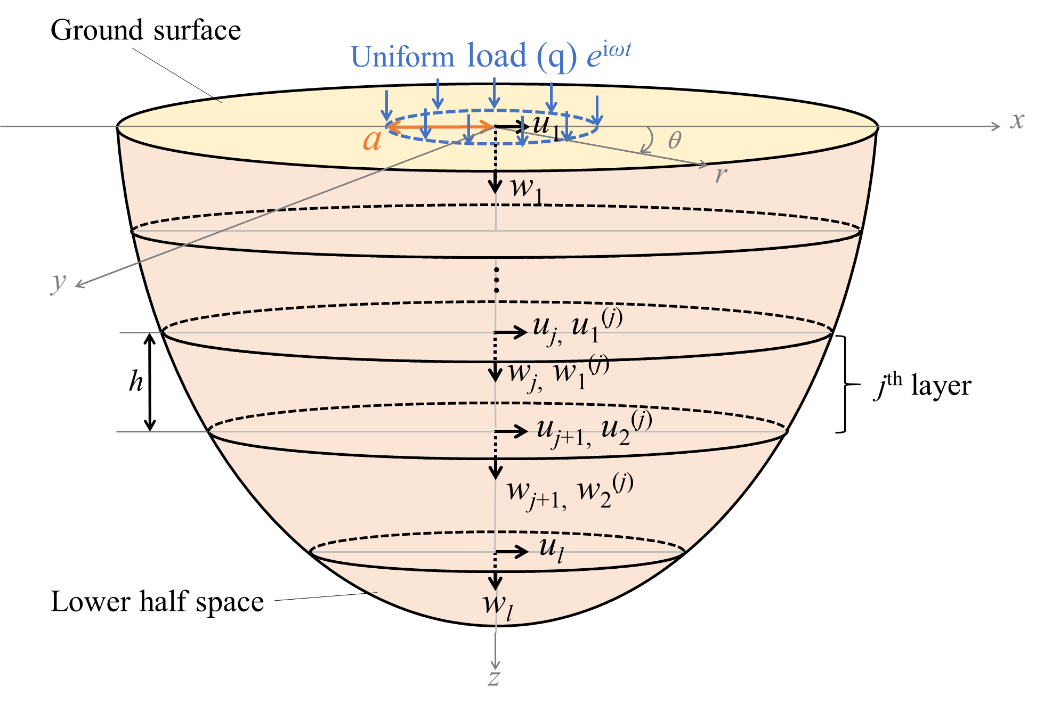
\includegraphics[scale=0.3]{images/earthmodel.png}
    \caption{The coordinates and variables in a layered half space.}
    \label{fig:earthmodel}
\end{figure}


Although extensive literature review in this proposal is set in the next part, here after in this part will be an important description of the current research from Geo-Imaging and Geo-Nerve Lab (GIGN Lab) led by Prof. Chih-Ping Lin. The current research plays an important part in the proposed research topic. Thus, I would like to describe Prof. Lin’s and his team's research in the introduction section.  

The Geo-Imaging and Geo-Nerve Lab (GIGN Lab), where I belong, has done various research on applying geophysical methods to characterize the geotechnical engineering parameters. Currently, Prof. Chih-Ping Lin in GIGN lab and his research team are developing a more efficient model called Full-Wavefield Computational Model based on Fourier-Bessel Expansion (FBE) which is accurate and time efficient. The research on the new framework of full-wavefield inversion using the data from multichannel analysis of surface waves and the analysis based on Fourier-Bessel expansion, the framework is more time efficient compared to others’ algorithms such as MultiSmart3D. The multi-layer model coordinate and model parameters are presented in figure \ref{fig:earthmodel}.

From the results of Lin and his research team, the proposed model (FBE model) outperforms the modal summation method because the Full-wavefield inversion based on FBE is able to deal with near-field effects and leaky waves, while the modal summation is less accurate when dealing with those problems.   
The dispersion images with different modes (fundamental and higher modes) of the vertical and horizontal components of both the FBE and MultiSmart3D are shown in figure \ref{fig:DCvertical} and figure \ref{fig:DChorz}.           

\begin{figure}[h]
    \centering
    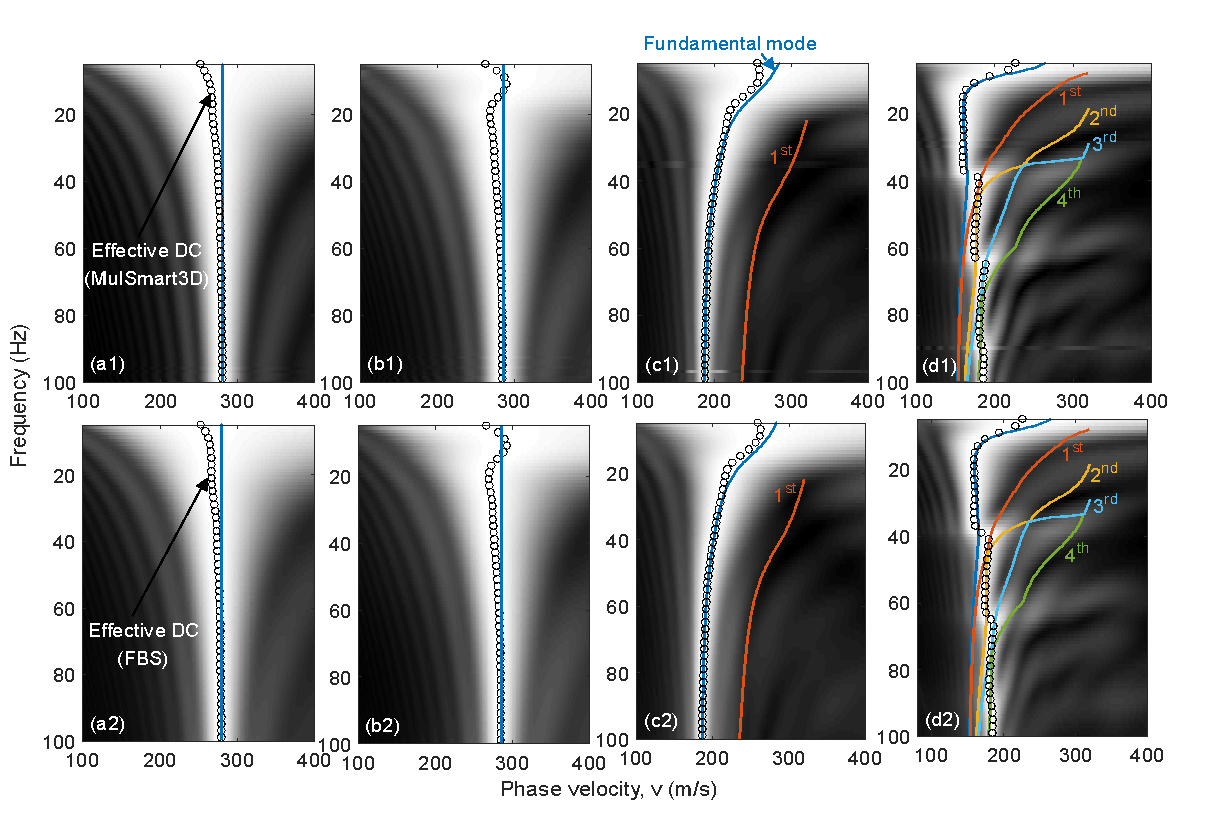
\includegraphics[scale=0.3]{images/DCvertical.png}
    \caption{Dispersion images and dispersion curves of the vertical component signal from different models: (a) homogeneous half space (Poisson's ratio=0.33); (b) homogeneous half space (Poisson's ratio=0.48); (c) 3-layered model; (d) 4-layered model. Results from MultiSmart3D are shown on the top whilst those from FBS on the bottom. The solid lines in the spectra are the theoretical modal dispersion curves.}
    \label{fig:DCvertical}
\end{figure}
\hfill
\begin{figure}[h]
    \centering
    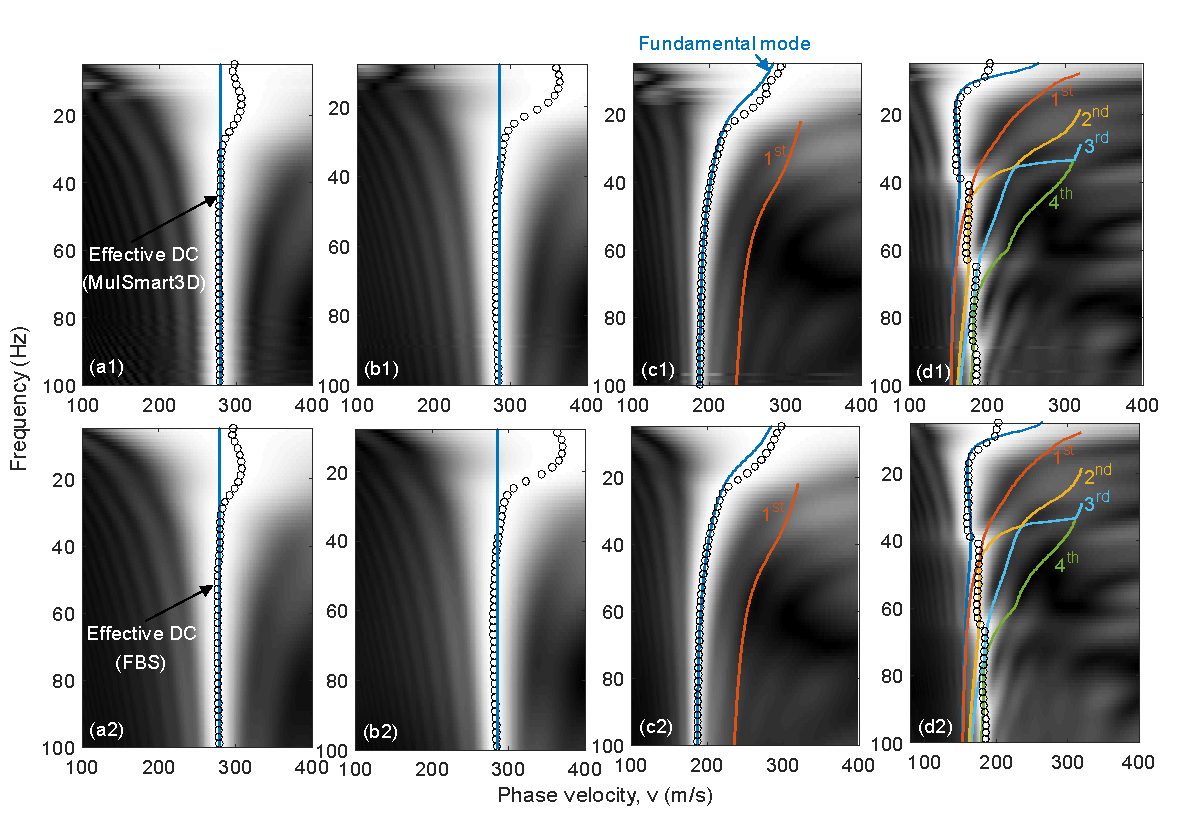
\includegraphics[scale=0.3]{images/DChorz.png}
    \caption{Dispersion images and dispersion curves of the radial component signal from different models: (a) homogeneous half space (Poisson's ratio=0.33); (b) homogeneous half space (Poisson's ratio=0.48); (c) 3-layered model; (d) 4-layered model. Results from MultiSmart3D are shown on the top whilst those from FBS on the bottom. The solid lines in the spectra are the theoretical modal dispersion curves.}
    \label{fig:DChorz}
\end{figure}

The research presented three pairs of shear wave velocity profiles to demonstrate the performance of full-wavefield inversion based on FBE shown in figure \ref{fig:VsAB},\ref{fig:VsCD}, and figure \ref{fig:VsEF}. There are several parameters used as information to indicate the level of uniqueness for the sake of shear wave velocity profiles inverted such as model dispersion curves, effective dispersion curves and dispersion spectra. 

\begin{figure}
    \centering
    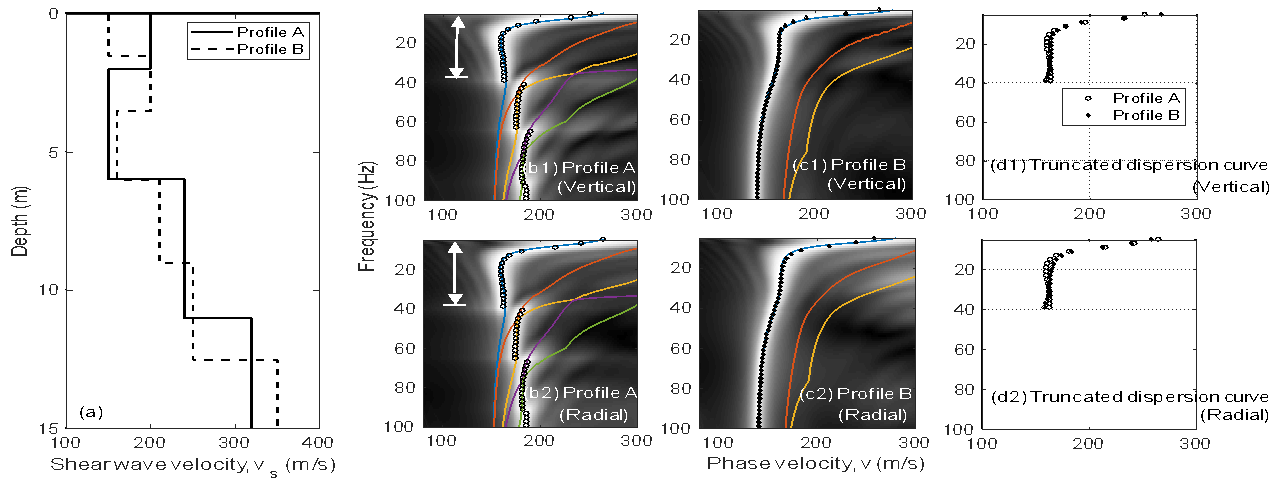
\includegraphics[scale=0.45]{images/VsAB.png}
    \caption{(a) The vs profiles; (b) the velocity spectra and effective dispersion curves of vertical component (top) and radial component (bottom) for profile A; (c) the velocity spectra and effective dispersion curves of vertical component (top) and radial component (bottom) for profile B; (d) comparison of the two fundamental-mode dispersion curves within the same frequency range for vertical component (top) and radial component (bottom). Lines in (b) and (c) are normal modes.}
    \label{fig:VsAB}
\end{figure}

Figure \ref{fig:VsAB} indicates the distinct dispersion curve corresponding to the two different Vs profiles (profile A and B). There is one feature that is interesting which is that the fundamental mode dispersion curve in range of frequency from 15-40 Hz looks very similar, but their corresponding velocity files are entirely different. Nonetheless, from the frequency higher than 40 Hz, the relations between fundamental dispersion curves and Vs of two profiles are complicated and hard to explain based only on fundamental dispersion curves.   

\begin{figure}
    \centering
    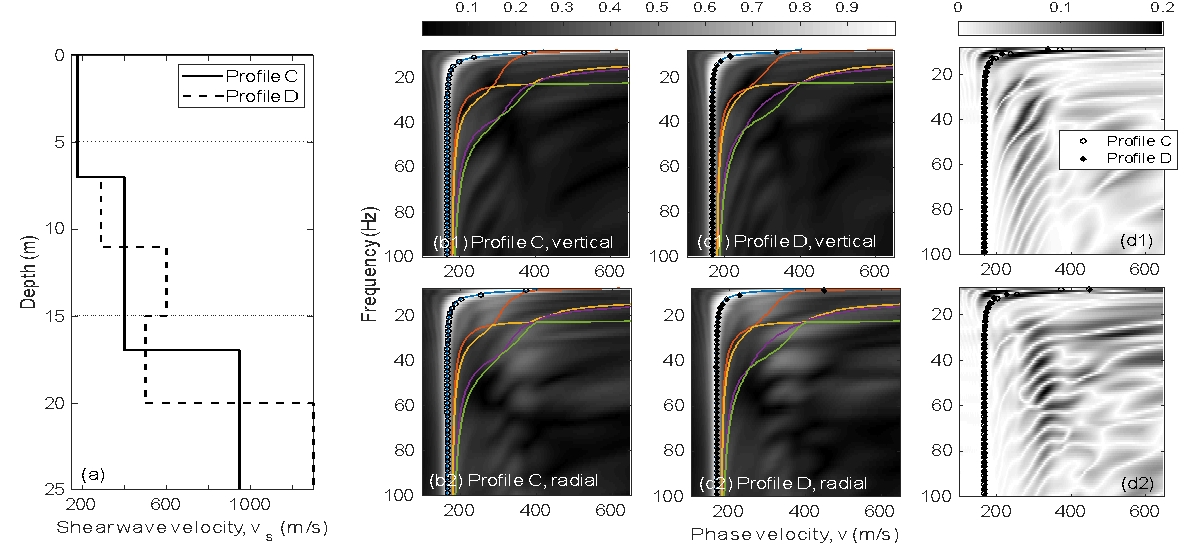
\includegraphics[scale=0.45]{images/VsCD.png}
    \caption{(a) The vs profiles; (b) the velocity spectra and effective dispersion curves of vertical component (top) and radial component (bottom) for profile C; (c) the velocity spectra and effective dispersion curves of vertical component (top) and radial component (bottom) for profile D; (d) comparison of the two effective dispersion curves and their velocity spectrum difference for vertical component (top) and radial component (bottom). Lines in (b) and (c) are normal modes.}
    \label{fig:VsCD}
\end{figure}

Figure \ref{fig:VsCD} demonstrates the very similar dispersion curves (cases of profile C and D), but the similarity in the velocity profiles are just within 0 to 7 m. If looking deeper, the velocity profiles are very different or even contrast, while the dispersion images are nearly identical observed in both fundamental and higher-order dispersion curves. Another point is the observation of the velocity spectrum images, which may contain meaningful information at the certain parts (frequency and velocity regions). In other words, we may be able to extract more information by looking in batches of dispersion data. The profile E and F presents the similar dispersion images and also the similar patents of velocity profiles, which is the increase Vs magnates in proportion to the increasing depth. The different of Vs profiles of E and F are the different Poisson’s ratio, in which (profile E has Poisson's ratio = 0.45 and profile F has Poisson's ratio = 0.3), the Vs magnitudes of profile F is close to that of E, but in higher depth, the Vs magnitudes of F is larger than that of E (from 10 m to deeper). Further observation is that the lower frequency effective dispersion curve is due to leaky waves (profile E), while the fundamental mode is dominant (profile F). Such that the performance fundamental mode inversion with respect to profile E may result in the overestimate in deep layer, the author suggested that making use of effective-mode inversion is much more appropriate than fundamental-mode inversion.

\begin{figure}
    \centering
    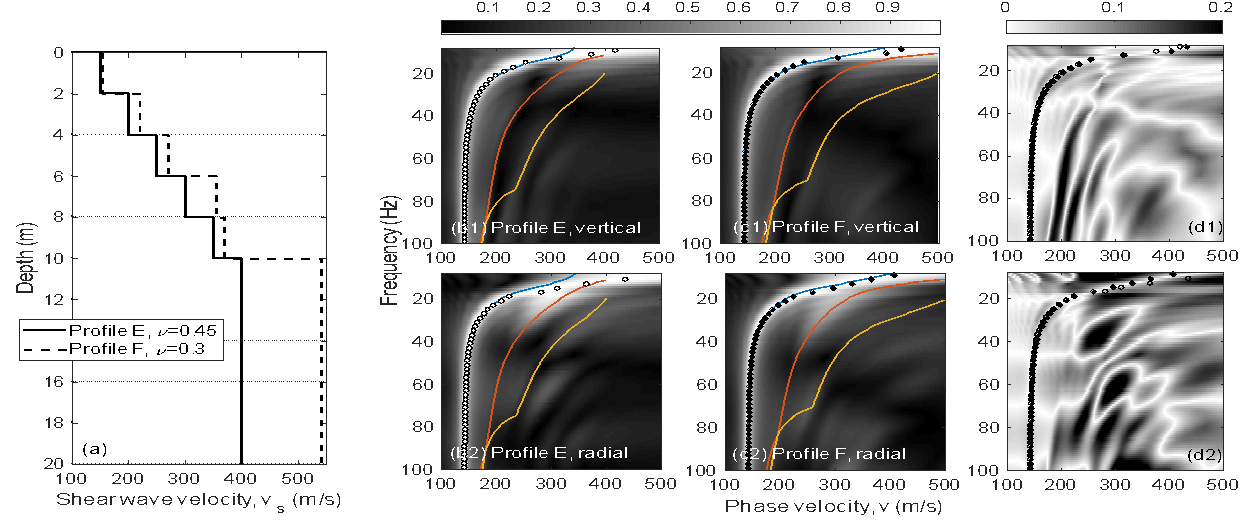
\includegraphics[scale=0.45]{images/VsEF.png}
    \caption{(a) The vs profiles; (b) the velocity spectra and effective dispersion curves of vertical component (top) and radial component (bottom) for profile E; (c) the velocity spectra and effective dispersion curves of vertical component (top) and radial component (bottom) for profile F; (d) comparison of the two effective dispersion curves and their velocity spectrum difference for vertical component (top) and radial component (bottom). Lines in (b) and (c) are normal modes.}
    \label{fig:VsEF}
\end{figure}

\begin{figure}
    \centering
    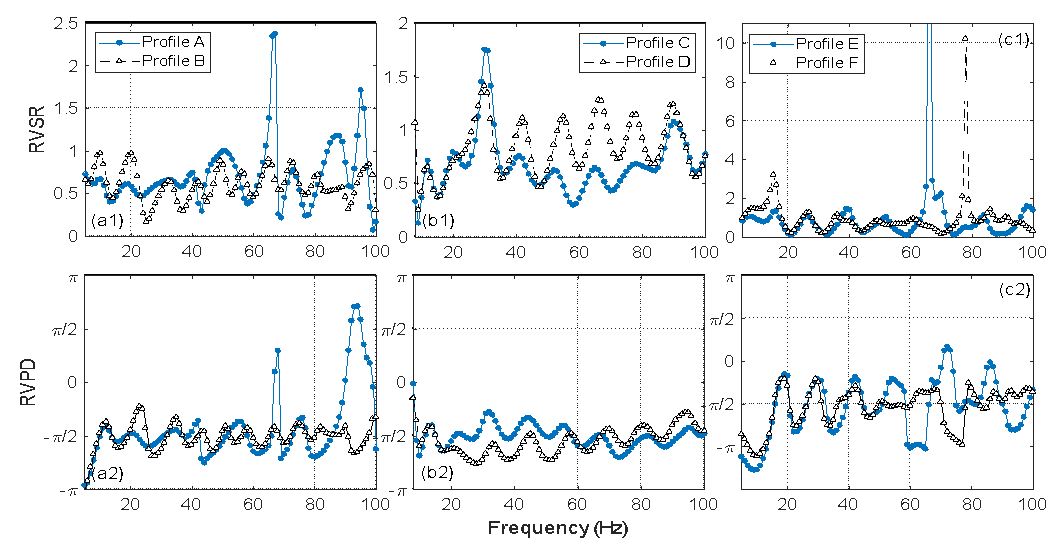
\includegraphics[scale=0.45]{images/RVSR.png}
    \caption{(RVSR (on top) and RVPD (on bottom) for the three pairs of cases at the middle receiver (offset = 28 m): (a) Profile A and B; (b) Profile C and D; (c) Profile E and F.}
    \label{fig:RVSR}
\end{figure}

Because of the occurrence of different scenarios in inversion problems, one possible way is to try to extract more features from the data through power density spectrum in time or frequency domain, dispersion images or velocity spectrum and phase different spectrum, or other possible features. Figure \ref{fig:RVSR} illustrates the radial-to-vertical spectral ratio between different profiles (RVSR) shown in top row and the radial-to-vertical phase difference of pairs of profiles (RVPD) shown in bottom row. The authors used the data at the middle receiver of 28 m offset. If we use data at all receivers, we may get the spectral images and those images may help to review much more meaning and explainable information.  

Currently, the results still contain non-uniqueness (different earth models may have similar fundamental modes or the apparent dispersion curves). Because of that, additional parameters for interpretation of inversion results have been introduced which are the radial to vertical spectral ratio and the phase difference. The research shows that the framework is able to take the take and perform dispersion analysis and inversion efficiently. Beyond that, more constraints have also been introduced which are very helpful to use information of seismograms images, dispersion curve images, spectral ratio, full velocity spectrum as the input of an artificial neural network as input data, then through the network, the output is the prediction of the velocity profiles of the classification of different modes dispersion curves. The concept of learning from data (deep learning) is based on the use of data feeding into a certain model to predict the target, or machine learning which requires less data as inputs into a model constituted by layers with the final layer as the output. The idea of using a new concept of deep learning (a subset of machine learning) can be applied in the inversion process with the training data is the known output, the error is the difference between the predicted result and actual result. The deep learning model can be used to compare with the traditional inversion analysis.

Although the newly developed inversion techniques still have some limitations, it provides a large and meaningful data. The future works can be done to remove those limitations and make the inversion process more reliable and really help the non-destructive method be a great technique in solving engineering problems. Because of the very fast development of artificial neural networks, the powerful computer available and the capability to collect huge amounts of data. The most common deep artificial neural networks are the Convolution Neural Networks (CNNs) and the Recurrence Neural Networks (RNNs). The CNNs are very powerful working with images (classifications, predictions), while RNNs are applicable for sequential signals (natural language processing). Currently, there are various powerful deep learning models and machine learning algorithms are developed and those models are used in multidisciplinary subjects (astronomy, geophysics, economics, robotics, artists …). The deep learning which is the combination of layers connected into a deep network with its parameters and hyper-parameters to take the input data and return desired output, the deep learning (DL) networks require much data, and the DL networks deal directly with input data. The machine learning (ML) models require manual manipulation of data (i.e., deal with the edges of images) then using the deep learning networks, usually require less data and there are plenty of ML models which can be combined to solve a certain problem. The DL networks are considered as a subset of ML, the ML models enable us to choose our own features, classifiers and training time with a small dataset. Both DL and ML are the cores of artificial intelligence (AI) models which come to perform tasks in the level far beyond what humans tell AI models to do. 

From the observations of the power and the potential of ANNs to solve the inversion problems. Specifically, the inversion of the geophysical properties to the geotechnical properties, which is then applied in the field of geotechnical engineering. Nowadays, the geophysical test is very popular all over the world involving various engineering applications and the data collected from geophysical are very large, it is because geophysical tests involve seismic wave or the electrical current, enable engineer to perform test in the large scale and the data acquisition process is automatic, therefore geophysical engineers are able to acquire a large amount of data from geophysical tests. Taking the advantages of the huge dataset from geophysical tests and the available ANNs, DL, ML models, we may have a lot to do with the dataset and we may be able to interpret the data in a way that has never been explained in the past. The non-uniqueness of inversion problems and the essence of ANNs that motivate me to propose a research to solve the non-uniqueness phenomenon in inversion problems. 
  
From above introduction, I would like to propose the new approach to use the available datasets and datasets from performing geophysical test, then apply different machine learning models to train the input geophysical datasets (geophysical parameters) and predict the engineering parameters (desire output). The model parameters (weights and inputs) and hyper-parameters (number of layers, learning rate, number of epochs, optimization algorithm, …) are modified to explore the most applicable architecture of ML models. Also, the result of ML model will then be used to compare with the traditional inversion solutions to observe the performance of ML model with the conventional inversion algorithms.

The new point and also the most important aspect of this proposed research is the utilizations of conventional inversion (such as full-wavefield inversion approaches) to apply the artificial neural networks (such as CNNs, RNNs, and GANs) to further extract the crucial features or the insights of the data measured from the field (earth sub-layered system). The later part is to use the neural networks in order to perform the inversion tasks using the extracted features (not all features from large scale of data). The proposed research is expected to provide a new breakthrough and a complement to the current studies on earth sub-layered inversion problems with higher resolution and accuracy compared to previous studies.